\PassOptionsToPackage{unicode}{hyperref}
\PassOptionsToPackage{naturalnames}{hyperref}
\documentclass{article}
\usepackage{geometry}
%\usepackage{fullpage}
\usepackage{parskip}
\usepackage{physics}
\usepackage{amsmath}
\usepackage{amssymb}
\usepackage{xcolor}
\usepackage[colorlinks,linkcolor=blue,citecolor=green]{hyperref}
\usepackage{array}
\usepackage{longtable}
\usepackage{multirow}
\usepackage{comment}
\usepackage{graphicx}
\usepackage{cite}
\usepackage{amsfonts}
\usepackage{bm}
\usepackage{slashed}
\usepackage{dsfont}
\usepackage{mathtools}
\usepackage[compat=1.1.0]{tikz-feynman}
\usepackage{simplewick}
%\usepackage{fourier}
%\usepackage{slashbox}
%\usepackage{intent}
\usepackage{mathrsfs}
\usepackage{xparse}
\usepackage{enumerate}
\usepackage{listings}

\geometry{left=0.9cm,right=0.9cm,top=1.5cm,bottom=2cm}

\newcommand{\gm}{\gamma^{\mu}}
\newcommand{\gn}{\gamma^{\nu}}
\newcommand{\gs}{\gamma^{\sigma}}
\newcommand{\gr}{\gamma^{\rho}}
\newcommand{\gnr}{g^{\nu\rho}}
\newcommand{\gmr}{g^{\mu\rho}}
\newcommand{\gms}{g^{\mu\sigma}}
\newcommand{\gns}{g^{\nu\sigma}}
\newcommand{\vbp}{\vb{p}}
\newcommand{\vbk}{\vb{k}}
\newcommand{\g}{\gamma}
\renewcommand{\a}{\alpha}
\renewcommand{\b}{\beta}
\renewcommand{\t}{\theta}
\newcommand{\la}{\lambda}
\newcommand{\p}{\phi}
\newcommand{\vp}{\varphi}
\newcommand{\s}{\sigma}
\renewcommand{\G}{\Gamma}
\newcommand{\pars}{\slashed\partial}
\newcommand{\ps}{\slashed p}
\newcommand{\ks}{\slashed k}
\newcommand{\bP}{\vb{P}}
\newcommand{\bA}{\vb{A}}
\newcommand{\ba}{\boldsymbol{\alpha}}
\newcommand{\apo}{\abs{\vb{p}_1}}
\newcommand{\aps}{\abs{\vb{p}_2}}
\newcommand{\lag}{\mathcal{L}}

\definecolor{mygray}{rgb}{0.9,0.9,0.9}
\lstset{
  frame=single,
  backgroundcolor=\color{mygray},
  extendedchars=true,
  language=Mathematica
}

\title{Homework: Particle Physics \#1}
\author{Yingsheng Huang}
\begin{document}
\maketitle
\begin{enumerate}[\bf1.]
  \item $\g^0(\gm)^{\dagger}\g^0=\gm$
  $$\g^0{\g^0}^{\dagger}\g^0=\g^0,\g^0{\g^i}^{\dagger}\g^0=2\delta^0_i-{\g^i}^{\dagger}=-{\g^i}^{\dagger}=\g^i$$
  $$\Longrightarrow \g^0(\gm)^{\dagger}\g^0=\gm\;\;\;\;\;\;\;\;\;\;\;\text{(Used ${\g^i}^{\dagger}=\g_i=-\g^i$)}$$
  \item From the orthogonal condition, we have the orthogonal condition of spinor $\xi$: $\xi^{\dagger}\xi=1$, then
  \begin{align*}
    \sum_su_s(p)\bar u_s(p)&=\sum_s\pmqty{\sqrt{p\cdot\sigma}\xi^s\\\sqrt{p\cdot\bar\sigma}\xi^s}\pmqty{\xi^{s\dagger}\sqrt{p\cdot\bar\sigma}&\xi^{s\dagger}\sqrt{p\cdot\sigma}}\\
    &=\sum_s\pmqty{\sqrt{p\cdot\sigma}\xi^s\xi^{s\dagger}\sqrt{p\cdot\bar\sigma}&\sqrt{p\cdot\sigma}\xi^s\xi^{s\dagger}\sqrt{p\cdot\sigma}\\\sqrt{p\cdot\bar\sigma}\xi^s\xi^{s\dagger}\sqrt{p\cdot\bar\sigma}&\sqrt{p\cdot\bar\sigma}\xi^s\xi^{s\dagger}\sqrt{p\cdot\sigma}}\\
    \intertext{(Use $\sum_s\xi^s\xi^{s\dagger}=\mathds{1}$)}
    &=\pmqty{m&p\cdot\sigma\\p\cdot\bar\sigma&m}\\
    &=\ps+m
  \end{align*}
  Similarly, $\sum_sv_s(p)\bar v_s(p)=\ps-m$.
  \item $m=0$, $k^{\mu}=\{k_0,k_x,k_y,k_z\}$, there's two transverse polarization vector, we can choose (note that the orthogonal and completeness conditions are also considered)
  $$k\cdot \epsilon=0\Longrightarrow \epsilon^1=\Pmqty{0,\frac{\sqrt{\text{ky}^2+\text{kz}^2}}{\sqrt{\text{kx}^2+\text{ky}^2+\text{kz}^2}},-\frac{\text{kx} \text{ky}}{\sqrt{\text{ky}^2+\text{kz}^2} \sqrt{\text{kx}^2+\text{ky}^2+\text{kz}^2}},-\frac{\text{kx} \text{kz}}{\sqrt{\text{ky}^2+\text{kz}^2} \sqrt{\text{kx}^2+\text{ky}^2+\text{kz}^2}}},\epsilon^2=\Pmqty{0,0,\frac{\text{kz}}{\sqrt{\text{ky}^2+\text{kz}^2}},-\frac{\text{ky}}{\sqrt{\text{ky}^2+\text{kz}^2}}}$$
  \item Consider a general transformation
  \begin{align*}
    f(x)\rightarrow f'(x')
  \end{align*}
  and define
  \begin{align*}
    \delta f\equiv f'(x')-f(x)=f'(x+\delta x^{\mu})-f(x)\cong f'(x)-f(x)+\delta x^{\mu}\partial_{\mu}f+\mathcal{O}(\delta x^2)
  \end{align*}
  and also define
  \begin{align*}
    \delta_0 f=f'(x)-f(x)
  \end{align*}
  then
  \begin{align*}
    \delta f=\delta_0 f+\delta x^{\mu}\partial_{\mu}f
  \end{align*}
  Now we deal with this problem from the least action principle first
  \begin{align*}
    &\delta S=0\\
    =&\int\dd^4x\delta\lag+\int\delta(\dd^4x)\lag
  \end{align*}
  And
  \begin{align*}
    \delta\lag&=\delta_0\lag+\delta x^{\mu}\partial_{\mu}\lag\\
    &=\pdv{\lag}{\phi}\delta_0\phi+\pdv{\lag}{(\partial_{\mu}\phi)}\delta_0(\partial_{\mu}\phi)+\delta x^{\mu}\partial_{\mu}\lag\\
    &=\delta x^{\mu}\partial_{\mu}\lag+(\pdv{\lag}{\phi}-\partial_{\mu}\pdv{\lag}{(\partial_{\mu}\phi)})\delta_0\phi+\partial_{\mu}(\pdv{\lag}{(\partial_{\mu}\phi)}\delta_0\phi)
  \end{align*}
  The other part
  \begin{align*}
    \delta(\dd^4x)&=\pdv{\delta x^{\mu}}{x^{\mu}}\dd^4x=\partial_{\mu}(\delta x^{\mu})\lag
  \end{align*}
  which can be derived by
  \begin{align*}
    \dd^4x'=\abs{\pdv{x'^{\mu}}{x^{\nu}}}\dd^4x=\abs{\pdv{(x^{\mu}+\delta x^{\mu})}{x^{\nu}}}\dd^4x=(1+\pdv{\delta x^{\mu}}{x^{\mu}})\dd^4x
  \end{align*}
  And the whole part of $\delta S$ becomes (applying Euler-Lagarange equation)
  \begin{align*}
    \delta S&=\int\dd^4x \delta x^{\mu}\partial_{\mu}\lag+(\pdv{\lag}{\phi}-\partial_{\mu}\pdv{\lag}{(\partial_{\mu}\phi)})\delta_0\phi+\partial_{\mu}(\pdv{\lag}{(\partial_{\mu}\phi)}\delta_0\phi)+ \partial_{\mu}(\delta x^{\mu})\lag\\
    &=\int\dd^4x \partial_{\mu}(\delta x^{\mu}\lag)+(\pdv{\lag}{\phi}-\partial_{\mu}\pdv{\lag}{(\partial_{\mu}\phi)})\delta_0\phi+\partial_{\mu}(\pdv{\lag}{(\partial_{\mu}\phi)}\delta_0\phi)\\
    &=\int\dd^4x \partial_{\mu}(\delta x^{\mu}\lag)+\partial_{\mu}(\pdv{\lag}{(\partial_{\mu}\phi)}\delta_0\phi)
  \end{align*}
  Note that $\delta_0 \phi=\delta \phi-\delta x^{\mu}\partial_{\mu}\phi$, and
  \begin{align*}
    \delta S&=\int\dd^4x \partial_{\mu}(\delta x^{\mu}\lag)+\partial_{\mu}(\pdv{\lag}{(\partial_{\mu}\phi)}\delta \phi-\pdv{\lag}{(\partial_{\mu}\phi)}\delta x^{\rho}\partial_{\rho}\phi)\\
    &=\int\dd^4x \partial_{\mu}\{\delta x^{\mu}\lag+\pdv{\lag}{(\partial_{\mu}\phi)}\delta \phi-\pdv{\lag}{(\partial_{\mu}\phi)}\delta x^{\rho}\partial_{\rho}\phi\}\\
    &=\int\dd^4x \partial_{\mu}\{(\lag g^{\mu}_{\rho}-\pdv{\lag}{(\partial_{\mu}\phi)}\partial_{\rho}\phi)\delta x^{\rho}+\pdv{\lag}{(\partial_{\mu}\phi)}\delta \phi\}
  \end{align*}
  \item Given
  $$P\psi P^{-1}=\eta\g^0\psi(t,-\vb{x})$$
  $$P\bar\psi P^{-1}=\eta^*\bar\psi(t,-\vb{x}) \g^0$$
  The field operators are
  $$\psi(x)=\int\frac{\dd^3p}{(2\pi)^3}\frac{1}{\sqrt{2E_{\vb{p}}}}\sum_s(a^s_{\vb{p}}u^s(p)e^{-ip\cdot x}+b^{s\dagger}_{\vb{p}}v^s(p)e^{ip\cdot x})$$
  $$\bar\psi(x)=\int\frac{\dd^3p}{(2\pi)^3}\frac{1}{\sqrt{2E_{\vb{p}}}}\sum_s(b^s_{\vb{p}}\bar v^s(p)e^{-ip\cdot x}+a^{s\dagger}_{\vb{p}}\bar u^s(p)e^{ip\cdot x})$$
  To satisfy the first two equations when acted on by P operator, the creation \& annihilation operators must obey
  $$Pa_{\vb{p}}^sP^{-1}=\eta a_{\vb{-p}}^s,Pb_{\vb{p}}^sP^{-1}=-\eta^* b_{\vb{-p}}^s$$
  (Note that $u(p^0,\vbp)=\g^0u(p^0,-\vbp)$, $v(p^0,\vbp)=-\g^0v(p^0,-\vbp)$)
  \item Given
  $$C\psi C^{-1}=-i(\bar\psi\g^0\g^2)^T=-i\g^2\psi^*$$
  $$C\bar\psi C^{-1}=-i(\g^0\g^2\psi)^T=i\bar\psi^*\g^2$$
  Similarly, the creation \& annihilation operators must obey
  $$Ca_{\vbp}^sC^{-1}=b_{\vbp}^s,Cb_{\vbp}^sC^{-1}=a_{\vbp}^s$$
  (Note that $u^s(p)=-i\g^2(v^s(p))^*$, $v^s(p)=-i\g^2(u^s(p))^*$)
  \item Prove Landau-Yang theorem.

	For any vector particles,we can always write the field operator as a single vector field.
  $$A_{\mu}(x)=\int\frac{\dd^3k}{(2\pi)^3}\frac{1}{\sqrt{2\abs{\vb{k}}}}\sum_{\la}(a^{\la}_{\vbk}\epsilon^{\la}_{\mu}(k)e^{-ik\cdot x}+{a^{\la}_{\vbk}}^{\dagger}{\epsilon^{\la}_{\mu}}^*(k)e^{ik\cdot x})$$
  Then the feynman rules can be easily derived. The amplitude of $vector\rightarrow \g\g$ is
  \begin{align*}
    i\mathcal{M}&=\epsilon_1^{*\mu}(p_1)\epsilon_2^{*\nu}(p_2)\epsilon^{\a}(p)\Gamma_{\mu\nu\s}\\
    \intertext{since it must obey Lorentz-invariant}
    &=(\epsilon_1\cdot\epsilon_2)(a_1\epsilon\cdot p_1+a_2\epsilon\cdot p_2)+a_3(\epsilon_1\cdot \epsilon)(\epsilon_2\cdot p_1)+a_4(\epsilon_2\cdot \epsilon)(\epsilon_1\cdot p_2)\\
    \intertext{final states symmetry (identical), $a_1=a_2$, first term vanishes. And $\epsilon_2\cdot p_1=\epsilon_1\cdot p_2=0$}
    &=0
  \end{align*}
  \item Tensor field.

  At lowest order, we can assume there's no propagator.
  $$i\mathcal{M}=\varepsilon_{\mu\nu}(p)(i\Gamma^{\mu\nu\rho\s}(k_1,k_2))\epsilon^*_{1\rho}(k_1)\epsilon^*_{2\s}(k_2)$$
  $\Gamma$ is the effective vertex.

  Use Lorenz covariance 
  $$i\mathcal{M}=\varepsilon\cdot (ak_1+bk_2)(ck_1+dk_2)(\epsilon_1\cdot\epsilon_2)+e(\epsilon_1\cdot k_2)(\varepsilon\cdot\epsilon_2k_1)+f(\epsilon_2\cdot k_1)(\varepsilon\cdot\epsilon_1k_2)+j\varepsilon^{\mu}_{\mu}(\epsilon_1\cdot\epsilon_2)$$
  with $\epsilon_1\cdot k_2=\epsilon_2\cdot k_1=0$,
  $$i\mathcal{M}=\varepsilon\cdot (ak_1+bk_2)(ck_1+dk_2)(\epsilon_1\cdot\epsilon_2)+j\varepsilon^{\mu}_{\mu}(\epsilon_1\cdot\epsilon_2)$$
  \item $n\rightarrow p+e^-+\bar\nu_e$.

  In centre-of-mass frame, the range is $0\sim \sqrt{(m_n-m_p)^2-m_e^2}$.
  \item \begin{enumerate}[(a).]
  \item Use natual units:
  $$\psi(r)=\frac{g_0}{4\pi r}e^{-rm}$$
  and the equation
  $$ (\laplacian -m^2)\psi=0$$
  Obviously if we put $\psi$ in the equation there's a $m^2$ factor cancelled with the original $m^2$, so $\psi $ is a root of the equation.

  If closer look is taken, the Laplacian part should be (the coefficients are neglected)
  $$\frac{m^2 e^{-m r}}{r}+\frac{2 e^{-m r}}{r^3}+\frac{2 m e^{-m r}}{r^2}+\frac{2 \left(-\frac{e^{-m r}}{r^2}-\frac{m e^{-m r}}{r}\right)}{r}=\frac{m^2 e^{-m r}}{r}$$
  \item Add the source
  $$ (\laplacian -m^2)\psi=J^{\mu}$$
    \end{enumerate}
  \item $\pi^0\rightarrow\g\g$.

  The quantum numbers $J^{PC}$ of $\pi$ is $0^{-+}$ with zero spin and orbital angular momentum while for $\g$ it's $1^{--}$ with spin 1. Assuming we don't know anything about $\pi$, the final state angular momentum gives $J(\pi)=J(\g\g)=L+S$ is even. Since $L$ is odd, the final state system parity is $P=(-)^{L=1}=-$. And $J(\pi)=0$ (can also be proved by Furry's theorem, $J(\pi)$ can't be 1).
  \item $e^+e^-\rightarrow\g^*\rightarrow J/\psi$.

  Assuming $\g-J/\psi$ vertex is $(-iag^{\mu\nu})$
  $$i\mathcal{M}^{sr\la}=i\frac{ea}{M^2}\bar v^s(p_1)\slashed \epsilon^{\la}(p_1+p_2)u^r(p_2)$$
  Use kinematics (centre-of-mass), and choose circular polarization
  $$\epsilon^0=(0,0,0,1),\epsilon^+=(0,1,i,1),\epsilon^-=(0,1,-i,1)$$
  and only $$M^{12+}=M^{21-}=\frac{2ae}{M}$$ don't vanish. So $J/\psi$ is circular polarized.
  \item $\rho\rightarrow\pi\pi$. $\rho$ is vector particle and $\pi$ is pesudoscalar particle.
  $$i\mathcal{M}=\feynmandiagram[baseline=(x.base),small,horizontal=a to x]{a[particle=$\rho$]--[photon,momentum=p]x--[scalar,momentum=$p_1$]b[particle=$\pi$],
  x--[scalar,momentum=$p_2$]c[particle=$\pi$]};=i(ap_1+bp_2)\cdot\epsilon_{\rho}(p)$$
  So
  $$\sum\abs{\mathcal{M}}^2=\sum[(ap_1+bp_2)\cdot\epsilon_{\rho}(p)]^2=a(p_1-p_2)^2\cross (I,I_3)$$
  \item In $2\rightarrow3$ decay, there're total 4 independent 4-momentums, so 5 Lorenz scalars.

  For n particles, there're $\frac{n(n-3)}{2}$.
  \item  3-particle decay phase space integrals can be derived as follows:

  First we know that the gengeral non-relativistic expression for N-body phase space is
  \begin{align}
    \dd n=(2\pi)^3 \prod_{i=1}^{N}\frac{\dd^3\vb{p}_i}{(2\pi)^3}\delta^3\pqty{\vb{p}_{a}-\sum_{i=1}^{N}\vb{p}_i}
  \end{align}
  where $\vb{p}_a$ is the momentum of the decaying particle. (This expression can be derived easily from the phase space volume of each particle.) According to Fermi's golden rule (and notice the $(2E_i)^{1/2}$ ratio difference between $\mathcal{M}_{fi}$ and $T_{fi}$), the decay rate can be written as
  \begin{align}
    \Gamma_{fi}=\frac{(2\pi)^4}{2E_a}\int\abs{\mathcal{M}_{fi}}^2\delta(E_a-\sum_{i=1}^NE_i)\delta^3(\vb{p}_a-\sum_{i=1}^N\vb{p}_i)\prod_{i=1}^N\frac{\dd^3\vb{p}_i}{(2\pi)^32E_i}
  \end{align}
  So for 3-particle decay the decay rate can be written as
  \begin{align*}
    \Gamma_{fi}=\frac{(2\pi)^4}{2E_a}\int\abs{\mathcal{M}_{fi}}^2\delta(E_a-E_1-E_2-E_3)\delta^3(\vb{p}_a-\vb{p}_1-\vb{p}_2-\vb{p}_3)\frac{\dd^3\vb{p}_1}{(2\pi)^32E_1}\frac{\dd^3\vb{p}_2}{(2\pi)^32E_2}\frac{\dd^3\vb{p}_3}{(2\pi)^32E_3}
  \end{align*}
  Now we consider it in the centre-of-mass frame of the decaying particle A, which means $E_a=m_a$ and $\vb{p}_a=0$. Through the integration of delta function and $\dd^3\vb{p}_3$, we have
  \begin{align*}
    \Gamma_{fi}&=\frac{(2\pi)^4}{2m_a}\int\abs{\mathcal{M}_{fi}}^2\delta(m_a-E_1-E_2-E_3)\delta^3(\vb{p}_1+\vb{p}_2+\vb{p}_3)\frac{\dd^3\vb{p}_1}{(2\pi)^32E_1}\frac{\dd^3\vb{p}_2}{(2\pi)^32E_2}\frac{\dd^3\vb{p}_3}{(2\pi)^32E_3}\\
    &=\frac{(2\pi)^4}{2m_a}\int\abs{\mathcal{M}_{fi}}^2\delta(m_a-E_1-E_2-E_3)\frac{\dd^3\vb{p}_1}{(2\pi)^32E_1}\frac{\dd^3\vb{p}_2}{(2\pi)^32E_2}\frac{1}{(2\pi)^32E_3}\\
    &=\frac{1}{2^4m_a(2\pi)^5}\int\frac{\abs{\mathcal{M}_{fi}}^2}{E_1E_2E_3}\delta(m_a-E_1-E_2-E_3)\dd^3\vb{p}_1\dd^3\vb{p}_2\\
    &=\frac{1}{2^4m_a(2\pi)^5}\int\frac{\abs{\mathcal{M}_{fi}}^2}{E_1E_2E_3}\delta(m_a-E_1-E_2-E_3)\dd^3\vb{p}_1\dd^3\vb{p}_2\\
    &=\frac{1}{2^4m_a(2\pi)^5}\int\frac{\abs{\mathcal{M}_{fi}}^2\abs{\vb{p}_1}^2\abs{\vb{p}_2}^2\dd p_1\dd(\cos\theta_1)\dd\phi_1\dd p_2\dd(\cos\theta_2)\dd\phi_2}{E_1E_2\sqrt{\abs{\vb{p}_1}^2+\abs{\vb{p}_2}^2+2\abs{\vb{p}_1}\abs{\vb{p}_2}\cos\theta_2+m_3^2}}\\
    &\;\;\;\;\;\;\;\;\;\;\;\;\;\;\;\;\;\;\;\;\;\;\;\;\;\;\;\;\;\;\;\;\;\;\;\;\;\;\;\;\;\;\;\;\;\;\;\;\;\;\;\;\;\;\;\;\;\;\;\;\;\;\;\;\;\;\;\;\;\;\;\delta(m_a-E_1-E_2-\sqrt{\abs{\vb{p}_1}^2+\abs{\vb{p}_2}^2+2\abs{\vb{p}_1}\abs{\vb{p}_2}\cos\theta_2+m_3^2})
  \end{align*}
  where $\theta_1$, $\phi_1$ and $\phi_2$ are independent of the integral and therefore can be integrated first. Note that
  \begin{align*}
    \frac{\dd \abs{\vb{p}_i}}{\dd E_i}=\frac{E_i}{\abs{\vb{p}_i}}
  \end{align*}
  which means
  \begin{align*}
    \dd \abs{\vb{p}_i}=\frac{E_i}{\abs{\vb{p}_i}}\dd E_i
  \end{align*}
  and mark the kernel of $\delta$ function as
  \begin{align*}
    f(\cos\theta_2)\equiv m_a-E_1-E_2-\sqrt{\abs{\vb{p}_1}^2+\abs{\vb{p}_2}^2+2\abs{\vb{p}_1}\abs{\vb{p}_2}\cos\theta_2+m_3^2}
  \end{align*}
  we have
  \begin{align*}
    f'(\cos\theta_2)=-\frac{2\apo\aps}{2\sqrt{\apo^2+\aps^2+2\apo\aps\cos\theta_2+m_3^2}}
  \end{align*}
  and the real root of $f(\cos\theta_2)=0$ is
  \begin{align*}
    \cos\theta'_2=\frac{(m_a-E_1-E_2)^2-m_3^2-\apo^2-\aps^2}{2\apo\aps}
  \end{align*}
  So we have
  \begin{align*}
    &\delta(m_a-E_1-E_2-\sqrt{\abs{\vb{p}_1}^2+\abs{\vb{p}_2}^2+2\abs{\vb{p}_1}\abs{\vb{p}_2}\cos\theta_2+m_3^2})\\
    =&\frac{\delta(\cos\theta_2-\cos\theta_2')}{\frac{2\apo\aps}{2\sqrt{\apo^2+\aps^2+2\apo\aps\cos\theta'_2+m_3^2}}}
  \end{align*}
  And the original formula becomes
  \begin{align*}
    \Gamma_{fi}&=\frac{8\pi^2}{2^4m_a(2\pi)^5}\int\frac{\abs{\mathcal{M}_{fi}}^2\abs{\vb{p}_1}^2\abs{\vb{p}_2}^2\dd p_1\dd p_2\dd(\cos\theta_2)}{E_1E_2\sqrt{\abs{\vb{p}_1}^2+\abs{\vb{p}_2}^2+2\abs{\vb{p}_1}\abs{\vb{p}_2}\cos\theta_2+m_3^2}}\frac{\delta(\cos\theta_2-\cos\theta_2')}{\frac{2\apo\aps}{2\sqrt{\apo^2+\aps^2+2\apo\aps\cos\theta'_2+m_3^2}}}\\
    &=\frac{1}{2^3m_a(2\pi)^3}\int\frac{\abs{\mathcal{M}_{fi}}^2\abs{\vb{p}_1}^2\abs{\vb{p}_2}^2\dd p_1\dd p_2}{E_1E_2\sqrt{\abs{\vb{p}_1}^2+\abs{\vb{p}_2}^2+2\abs{\vb{p}_1}\abs{\vb{p}_2}\cos\theta'_2+m_3^2}}\frac{2\sqrt{\apo^2+\aps^2+2\apo\aps\cos\theta'_2+m_3^2}}{2\apo\aps}\\
    &=\frac{1}{2^3m_a(2\pi)^3}\int\frac{\abs{\mathcal{M}_{fi}}^2\abs{\vb{p}_1}\abs{\vb{p}_2}\dd p_1\dd p_2}{E_1E_2}\\
    &=\frac{1}{2^3m_a(2\pi)^3}\int\frac{\abs{\mathcal{M}_{fi}}^2\abs{\vb{p}_1}\abs{\vb{p}_2}\frac{E_1}{\abs{\vb{p}_1}}\dd E_1\frac{E_2}{\abs{\vb{p}_2}}\dd E_2}{E_1E_2}\\
    &=\frac{1}{8m_a(2\pi)^3}\int\abs{\mathcal{M}_{fi}}^2\dd E_1\dd E_2
  \end{align*}
  which is exactly the form of square Dalitz plot. Transform it a little bit and we have the standard form of Dalitz plot (note that $s_2=(p_2+p_3)^2=(p_a-p_1)^2\rightarrow\dd s_2=-2m_a\dd E_1$ and similar for $s_3$)
  \begin{align*}
    \Gamma_{fi}&=\frac{1}{32m_a(2\pi)^3}\int\abs{\mathcal{M}_{fi}}^2\dd s_2\dd s_3
  \end{align*}
  Now let's review another form of the standard Dalitz form
  \begin{align*}
    \frac{\dd\Gamma_{fi}}{\dd s_2\dd s_3}=\frac{1}{32m_a(2\pi)^3}\abs{\mathcal{M}_{fi}}^2
  \end{align*}
  and its physical meaning is obvious: the density of data points on a Dalitz plot is proportional to the decay matrix element.
  \item $J^{PC}(^{2S+1}L_J)$ of $q\bar q$ system. ($P=(-)^{L+1}$, $C=(-)^{L+S}$)

  $$\begin{array}{cccc}
    L\backslash S&0&1\\
    0&0^{-+}(^1S_0)&1^{--}(^3S_1)\\
    1&1^{+-}(^1P_1)&0^{++}(^3P_0)\\&&1^{++}(^3P_1)\\&&{2^{++}}(^3P_2)\\
    2&2^{-+}(^1D_2)&1^{--}(^3D_1)\\&&2^{--}(^3D_2)\\&&3^{--}(^3D_3)
  \end{array}$$
  \item Moller scattering.

  Use FeynCalc.
  \begin{lstlisting}
    <<FeynCalc`;
    topMoeller = CreateTopologies[0, 2 -> 2];
    diagsMoeller = InsertFields[topMoeller, {F[2, {1}], F[2, {1}]} -> {F[
			2, {1}], F[2, {1}]}, InsertionLevel -> {Classes}, Model -> "SM",
			ExcludeParticles -> {S[1], S[2], V[2]}];
    Paint[diagsMoeller, ColumnsXRows -> {2, 1}, Numbering -> None,
      SheetHeader->None,ImageSize->{512,256}];
  \end{lstlisting}
  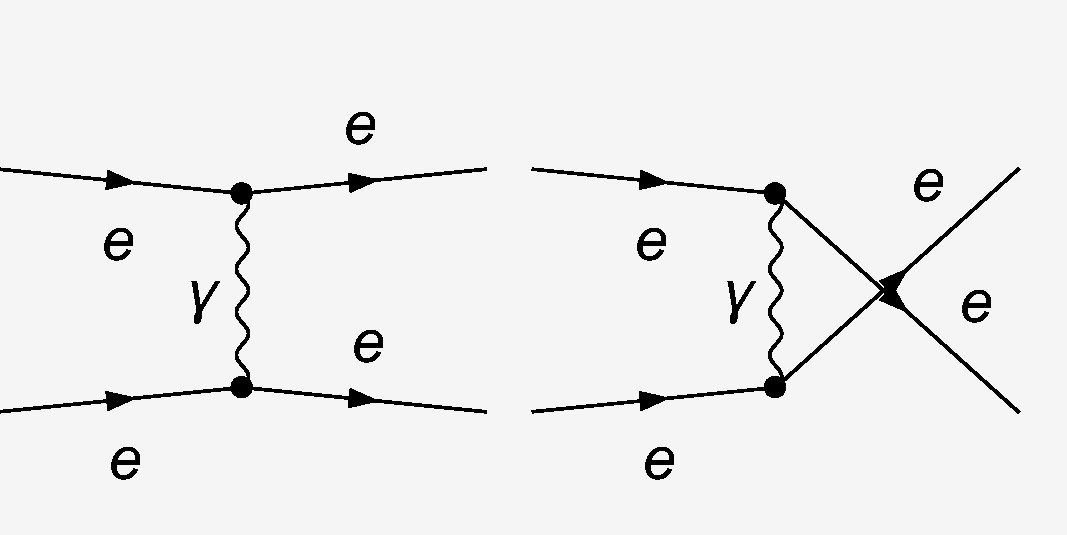
\includegraphics[height=3cm]{QEDMoellerScatteringTree.pdf}
  \begin{lstlisting}
    ampMoeller=FCFAConvert[CreateFeynAmp[diagsMoeller, Truncated -> False],
      IncomingMomenta->{p1,p2},OutgoingMomenta->{k1,k2},UndoChiralSplittings->True,
      ChangeDimension->4,List->False,SMP->True]
  \end{lstlisting}
  \begin{align*}
    i\mathcal{M}&=\frac{\bar{g}^{\text{Lor1}\text{Lor2}} \left(\varphi (\overline{\text{k1}},m_e)\right).\left(i
   \text{e} \bar{\gamma }^{\text{Lor1}}\right).\left(\varphi (\overline{\text{p1}},m_e)\right)
   \left(\varphi (\overline{\text{k2}},m_e)\right).\left(i \text{e} \bar{\gamma
   }^{\text{Lor2}}\right).\left(\varphi
   (\overline{\text{p2}},m_e)\right)}{\left(\overline{\text{k2}}-\overline{\text{p2}}\right)^2
   }\\&-\frac{\bar{g}^{\text{Lor1}\text{Lor2}} \left(\varphi
   (\overline{\text{k1}},m_e)\right).\left(i \text{e} \bar{\gamma
   }^{\text{Lor2}}\right).\left(\varphi (\overline{\text{p2}},m_e)\right) \left(\varphi
   (\overline{\text{k2}},m_e)\right).\left(i \text{e} \bar{\gamma
   }^{\text{Lor1}}\right).\left(\varphi
   (\overline{\text{p1}},m_e)\right)}{\left(\overline{\text{k1}}-\overline{\text{p2}}\right)^2
   }
  \end{align*}
  \begin{lstlisting}
    SetMandelstam[s, t, u, p1, p2, -k1, -k2, SMP["m_e"], SMP["m_e"], SMP["m_e"], SMP["m_e"]];
    sqAmpMoeller =(ampMoeller (ComplexConjugate[ampMoeller]//FCRenameDummyIndices))//
	PropagatorDenominatorExplicit//Contract//FermionSpinSum[#, ExtraFactor -> 1/2^2]&//
	ReplaceAll[#, DiracTrace :> Tr] & // Contract//Simplify
  \end{lstlisting}
  $$\sum\abs{\mathcal{M}}^2=\frac{2 \text{e}^4 \left(-4 m_e^2 \left(s \left(t^2+3 t u+u^2\right)+t^3-2 t^2 u-2 t
   u^2+u^3\right)+8 m_e^4 \left(t^2+t u+u^2\right)+s^2 (t+u)^2+t^4+u^4\right)}{t^2 u^2}$$
   And the differential cross section is
   $$\dv{\s}{\Omega}=\frac{\abs{\mathcal{M}^2}}{64\pi^2E_{cm}^2}$$
  \item Bhabha scattering.
  Similarily, use FeynCalc.
  \begin{lstlisting}
    <<FeynCalc`;
    topBhabha = CreateTopologies[0, 2 -> 2];
    diagsBhabha = InsertFields[topBhabha, {F[2, {1}], -F[2, {1}]} ->
		  {F[ 2, {1}], -F[2, {1}]}, InsertionLevel -> {Classes},
		    Model -> "SM", ExcludeParticles -> {S[1], S[2], V[2]}];
    Paint[diagsBhabha, ColumnsXRows -> {2, 1}, Numbering -> None,SheetHeader->None,
      ImageSize->{512,256}];
  \end{lstlisting}
  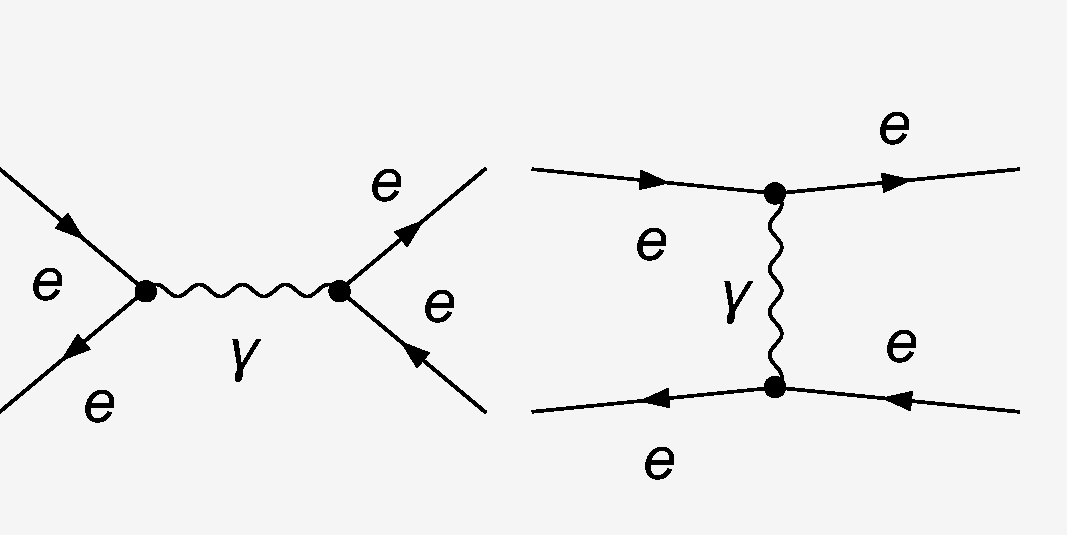
\includegraphics[height=3cm]{QEDBhabhaScatteringTree.pdf};
  \begin{lstlisting}
    ampBhabha=FCFAConvert[CreateFeynAmp[diagsBhabha, Truncated -> False],
    IncomingMomenta->{p1,p2},OutgoingMomenta->{k1,k2},UndoChiralSplittings->True,ChangeDim  ension->4,List->False, SMP->True]
  \end{lstlisting}
  \begin{align*}
    i\mathcal{M}&=\frac{\bar{g}^{\text{Lor1}\text{Lor2}} \left(\varphi (\overline{\text{k1}},m_e)\right).\left(i
   \text{e} \bar{\gamma }^{\text{Lor2}}\right).\left(\varphi
   (-\overline{\text{k2}},m_e)\right) \left(\varphi (-\overline{\text{p2}},m_e)\right).\left(i
   \text{e} \bar{\gamma }^{\text{Lor1}}\right).\left(\varphi
   (\overline{\text{p1}},m_e)\right)}{\left(\overline{\text{k1}}+\overline{\text{k2}}\right)^2
   }\\&-\frac{\bar{g}^{\text{Lor1}\text{Lor2}} \left(\varphi
   (\overline{\text{k1}},m_e)\right).\left(i \text{e} \bar{\gamma
   }^{\text{Lor1}}\right).\left(\varphi (\overline{\text{p1}},m_e)\right) \left(\varphi
   (-\overline{\text{p2}},m_e)\right).\left(i \text{e} \bar{\gamma
   }^{\text{Lor2}}\right).\left(\varphi
   (-\overline{\text{k2}},m_e)\right)}{\left(\overline{\text{k2}}-\overline{\text{p2}}\right)^
   2}
  \end{align*}
  \begin{lstlisting}
    SetMandelstam[s, t, u, p1, p2, -k1, -k2, SMP["m_e"], SMP["m_e"], SMP["m_e"], SMP["m_e"]];
    sqAmpBhabha =
		(ampBhabha (ComplexConjugate[ampBhabha]//FCRenameDummyIndices))
    //PropagatorDenominatorExplicit//
		Contract//FermionSpinSum[#, ExtraFactor -> 1/2^2] & //ReplaceAll[#,
     DiracTrace :> Tr]&//Contract//Simplify
    masslessSqAmpBhabha = (sqAmpBhabha /. {SMP["m_e"] -> 0})//Simplify
  \end{lstlisting}
  $$\sum\abs{\mathcal{M}}^2=\frac{2 \text{e}^4 \left(s^4+s^2 u^2+2 s t u^2+t^4+t^2 u^2\right)}{s^2 t^2}$$
  And the differential cross section is
  $$\dv{\s}{\Omega}=\frac{\abs{\mathcal{M}^2}}{64\pi^2E_{cm}^2}$$
  \item Mott scattering. (Assuming the scalar-photon vertex is $ig(k_1-k_2)^{\mu}$, ignore electron mass.)
  \begin{align*}
    i\mathcal{M}=\feynmandiagram[inline=(x.base),small,vertical=y to x]{a--[fermion,momentum=$p_1$]x--[fermion,momentum=$p_2$]b,c--[scalar,momentum=$k_2$]y--[scalar,momentum=$k_1$]d,x--[photon]y};=ige\bar u(p_2)\gm u(p_1)\frac{1}{(p_2-p_1)^2+i\epsilon}(k_1-k_2)_{\mu}
  \end{align*}
  $$\frac{1}{4}\sum\abs{\mathcal{M}}^2=\frac{g^2e^2}{(p_2-p_1)^4}[2(k_1-k_2)\cdot p_{1}(k_1-k_2)\cdot p_{2}-(k_1-k_2)\cdot(k_1-k_2)p_{1}\cdot p_{2}]$$
  Use kinematics:
  \begin{align*}
    \frac{1}{4}\sum\abs{\mathcal{M}}^2&=\frac{g^2e^2}{(p_2-p_1)^4}[2(k_1-k_2)\cdot p_{1}(k_1-k_2)\cdot (k_1-k_2+p_1)]-\frac{g^2e^2}{(p_2-p_1)^2}[p_{1}\cdot (k_1+p_1-k_2)]\\
    &=\frac{2g^2e^2}{(p_2-p_1)^4}[p_2\cdot p_{1}]^2+\frac{g^2e^2}{(p_2-p_1)^2}[p_2\cdot p_{1}]\\
    &=\frac{2g^2e^2}{(p_2-p_1)^2}[p_2\cdot p_{1}]\\
    &=4g^2e^2
  \end{align*}
  The cross section is
  $$\dv{\s}{(\cos\theta)}=\frac{1}{2k^0_12p^0_1\abs{v_{k1}-v{p1}}}\frac{1}{16\pi}\frac{2\abs{p_1}}{E_{cm}}\abs{\mathcal{M}}^2$$
  \item Form factor.
  $$F^E(q^2)=\frac{1}{e}\int\dd^3r\rho(r)e^{iq\cdot r}=\frac{2\pi}{ e}\int\dd r\dd \theta\rho(r)e^{iqr\cos\theta}r^2\sin\theta$$
  $$F^E(q^2)=1-\frac{\abs{q}^2}{6}\expval{r^2}$$
  if no angular part, $\expval{r^2}\equiv\frac{1}{e}\int\dd^3r\rho(r)r^2=\frac{4\pi}{e}\int\dd r\rho(r)r^4$.

  $\rho(r)=\delta{(r)}$:
  $$F^E(q^2)=1$$
  $\rho(r)=\frac{\a^2}{4\pi}\frac{e^{-\a r}}{r}$:
  $$F^E(q^2)=\frac{\a^2}{\alpha ^2+q^2}=1-\frac{\abs{q}^2}{\a^2}$$
  $\rho(r)=\frac{m^3}{8\pi}e^{-m r}$:
  $$F^E(q^2)=\frac{ m }{\left(m ^2+q^2\right)^2}=1-\frac{2\abs{q}^2}{m^2}$$
  \item CP eigenvalues of $K^0\rightarrow\pi\pi$ \& $K^0\rightarrow\pi\pi\pi$ ($CP=(-)^{S-2s}$ for neutral system).

  For $2\pi$ system obviously they're all positive.

  For $3\pi$ system, consider $\pi^0\pi^0\pi^0$, $CP=(+)(-)^L(-)=(-)^{L+1}$ where $L$ is the orbital angular momentum between a $\pi^0\pi^0$ system and the other $\pi^0$. Also consider $\pi^+\pi^-\pi^0$, $CP=(-)^{L+1}$ where $L$ is the orbital angular momentum between a $\pi^+\pi^-$ system and $\pi^0$.
  \item Meson mass.

  From Gell-Mann-Okubo formula
  $$M(I,Y)=A+CY+B(I(I+1)-\frac{1}{4}Y^2)$$
  Take $J^P=0^-$, we have
  \begin{align*}
	M(K)=M(\frac{1}{2},1)=A+\frac{1}{2}B\\
    M(\pi)=M(1,0)=A+2B\\
    M(\bar K)=M(\frac{1}{2},-1)=A+\frac{1}{2}B\\
    M(\eta)=M(0,0)=A
  \end{align*}
  so
  $$4m^2_K=3m_{\eta_s}^2+m_{\pi}^2$$
  Experiments give a deviation of $6\%$.
  \item $e^+e^-\rightarrow\mu^+\mu^-$ and $e^+e^-\rightarrow J/\psi\rightarrow\mu^+\mu^-$.

  Check Peskin 5.1, the unpolarized cross section is
  $$\s=\frac{4\pi\a^2}{3E_{cm}^2}\sqrt{1-\frac{m_{\mu}^2}{E^2}}(1+\frac{1}{2}\frac{m_{\mu}^2}{E^2})$$
  and for $J/\psi$ production we need to work with the propagator: 

  add resonance structure to the propagator, it becomes (in Feynman gauge)
  $$\frac{-g^{\mu\nu}}{p^2-(m_{J/\psi}+i\frac{\Gamma}{2})^2}$$
  \item Use CP invariance (if not violated) to determine P parity of strange particles via weak interaciton.
\end{enumerate}




\end{document}
